\documentclass[a4paper,10pt]{article}

\usepackage{chin-report}
\usepackage{amsmath, amsthm}

\begin{document}
\fontfamily{lmss}\selectfont

{
	\small
    \hspace*{-0.3cm}  
    \begin{tabularx}{168mm}{ l X|X r }
        %\hline
        \multirow{7}{*}{
\includegraphics[width=9.8cm]{unilogo}} & & & BIO-4371 \\
	    & & & \textcolor{UT_RED}{\textbf{Structure-Based Drug Design}}  \\ [2pt]
        & & & Summer Semester 2025 \\
        & & & \\
        & & & Institute for Bioinformatics \\
        & & & and Medical Informatics \\
        %\hline
    \end{tabularx}
}

\begin{huge}
	\vspace{1cm}
	\textbf{Assignment Sheet 4}
\end{huge} \\

Authors: Mona Scheurenbrand, Mattes Warning, and Sarah Hüwels


\begin{large}
	\vspace{1.0cm}
	\textbf{A.4.1: Two Faces of Drug Chemistry}
\end{large}	\\ [2mm]
\textbf{1. [1 pt] What is (are) the most common name(s) for this category?} \\
Biologics

\textbf{2. [1 pt] This category contains a range of different product types. Give at least three different types.} \\
Vaccines, Tissues, Recombinant proteins (Antibodies)

\textbf{3. [1 pt] Select one exemplary type and explain it briefly (max. 180 words).} \\
Antibodies are proteins used by the adaptive immune system (AIS) to bind antigens. From the three classes of molecules used by the AIS, Antibodies recognize the widest range of antigenic structures and bind them strongest. In the following, we discuss the structural features of monoclonal antibodies. \\ \\
Monoclonal antibodies are Y-shaped proteins that have a symmetric core structure. They are composed of two identical light (L) and heavy (H) chains each of which can be further broken down into some constant (CL, CH) and one variable (VL, VH) domain. The variable domain of one heavy and one light chain forms an antigen-binding site. Each variable chain consists of a rather fixed framework region and three hypervariable or complementarity-determining regions (CDRs). We refer to the first, second, and third CDR of the antibody variable heavy chain as CDR-H1, CDR-H2, and CDR-H3 respectively.  CDRs are the main determinants of antigen binding and neutralization due to their high variability with CDR-H3 being the largest and most flexible.

\textbf{4. [1 pt] Please name a few major challenges in the development of these drug types that are less important in
small-molecule drug development?} \\
Pose generation, identification of pockets, binding affinity prediction, ligand binding optimization,

\begin{large}
	\vspace{1.0cm}
	\textbf{A.4.2: Target ID: Assessing Drugability}
\end{large}	\\ [2mm]
\textbf{1. Remove water and non-polymeric entities} \\
remove resn HOH \\
remove not polymer \\



\textbf{6. Please describe the approach that is used to calculate the ’druggability score’ briefly (max. 150 words).} \\
In the first step, pockets are identified using the detection algorithm DoGSite, which also calculates more than 40 global descriptors per pocket.
The most important of these descriptors are selected using shrinkage discriminant analysis. The druaggability score is then calculated from these descriptors using a SVM.
The SVM was trainined on the NRDD (druggability dataset). Outputs are between zero and one. The closer to the respective end, the higher the prediction confidence.

\textbf{7. Now, please inspect the results in order to find out if H. pylori urease is druggable. You may use the ’drug
score’ (= ’druggability score’) as an indicator for druggability. Apply a meaningful cutoff to select druggable
binding pockets (if existent). Please document your results and reasoning in the report.} \\
We used 0.7 as druggability score cutoff. In the paper they used 0.5 but we only had one pocket with druggability score
of 0.51 and the next highest score was 0.71. Because of this jump of 0.2 point we decided to omit the pocket with a score of 0.51.
0.71 is the next plausible threshold. The six identified pockets are: P0, P1, P2, P3, P4, P6.

\textbf{10. Copy one urease chain with bound inhibitor into a new object and align it onto your cleaned structure 1e9z.} \\
We visually inspected the structure to find a chain with bound ligand. We then removed all other chains: remove not chain T

\textbf{11. Please find out if one of the predicted pockets (partially) matches the experimentally observed binding pocket.
If yes, please create a meaningful visualization showing the ligand and the pocket residues and their location
in the protein chain. Store the result as scene F1 and save your PyMOL session.} \\
structures are aligned using: align 1e9z$\_$cleaned, 6zja

\begin{figure}[h!]
	\centering
	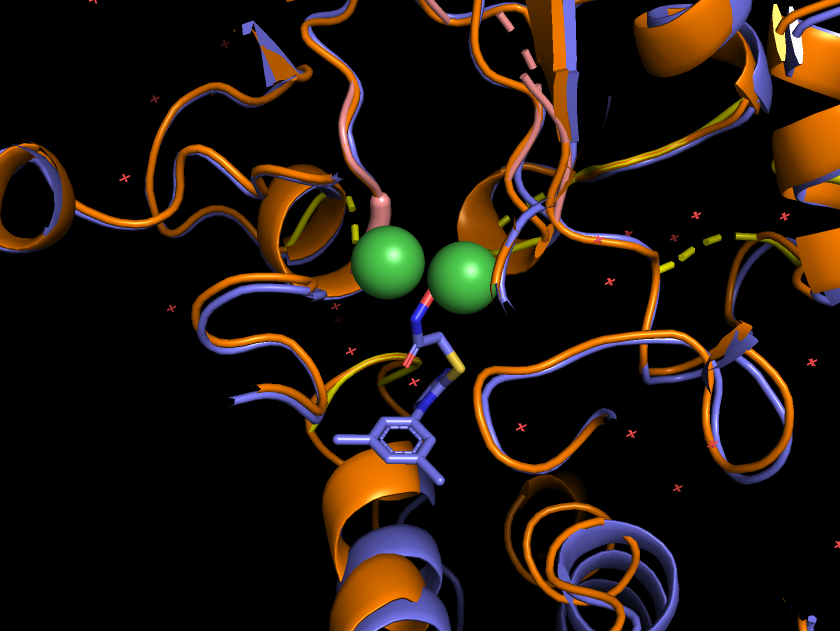
\includegraphics[width=0.5\linewidth]{A4.2_11}
	\caption{Pocket 3 (yellow) matches the experimentally observed binding pocket (purple). }
\end{figure}

\begin{large}
	\vspace{1.0cm}
	\textbf{A.4.3: Lead ID: HTS Data Analysis}

\end{large}	\\ [2mm]


Please refer to $A4_3$.ipynb for implementation details.

\bibliographystyle{plain}
\bibliography{bib}

\end{document}
